Ocurre cuando las ondas se \textbf{superponen en fase}, es decir, que estan alineadas en crestas y valles. Esto resulta en una onda con \textbf{mayor amplitud}. Tiene un efecto de \textbf{amplificación} entre las ondas.

\begin{figure}[H]
  \centering
  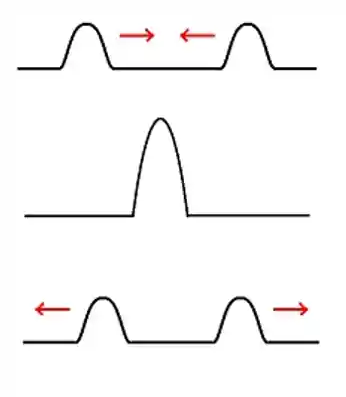
\includegraphics[scale=0.4]{imagenes/interferencia_constructiva.png}
  \caption{Interferencia destructiva\cite{respaionterf}}
\end{figure}
